\documentclass[t,aspectratio=169]{beamer}

\usepackage{bm}
\usepackage{soul}
\usepackage{tikz}
\usepackage{tikz-3dplot}
\usepackage{amsmath}
\usepackage{amsfonts}
\usepackage{amssymb}
%\usepackage{physics}
%\usepackage{graphicx}
\usepackage{multicol}
\usepackage[utf8]{inputenc}
\usepackage[magyar]{babel}

\usetikzlibrary{calc,3d,decorations.pathmorphing,decorations.pathreplacing,decorations.markings,snakes,arrows.meta,calc,patterns
}
\tikzset{snake it/.style={decorate, decoration=snake}}
% \usetheme{Madrid}
% \usecolortheme{whale}

% ----------------------------------------------------------------------------------------------------------------------------------------

\title{\includegraphics[width=45pt]{oepecsetlogo.png}\\(KTXFI1EBNF) Physics I. Lecture}

\author{Dr.~Gábor FACSKÓ, PhD\\\tiny Assistant Professor / Senior Research Fellow\\\textit{facsko.gabor@uni-obuda.hu}}

\institute{\Tiny Óbuda University, Faculty of Electrical Engineering, 1084 Budapest, Tavaszmező u. 17.\\Wigner Research Centre for Physics, Department of Space Physics and Space Technology, 1121 Budapest, Konkoly-Thege Miklós út 29–33.\\ \url{https://wigner.hu/~facsko.gabor}}

\date{March~16,~2026}

\logo{\includegraphics[height=0.9 true cm]{kekcsik.png}}

% ----------------------------------------------------------------------------------------------------------------------------------------

\begin{document}

\frame{\titlepage}

% ----------------------------------------------------------------------------------------------------------------------------------------

\begin{frame}
\frametitle{Current Updates and Issues}
\begin{itemize}
\setlength{\parskip}{0pt}
\setlength{\itemsep}{4pt}
\item Course materials (lecture and practice) are now available on Moodle, YouTube, and GitHub.
\item Homework No.~1 has been released (Deadline: March 22, 2026, midnight). Supplementary material is provided to assist you.
\item Please email your assignment to \texttt{facsko.gabor@uni-obuda.hu} as a \textbf{handwritten, scanned PDF}.
\item Proposed midterm exam: \textbf{May~11,~2026}. Retake: \textbf{May~18,~2026}.
\end{itemize}
\end{frame}

% ----------------------------------------------------------------------------------------------------------------------------------------

\begin{frame}[fragile,squeeze,allowframebreaks]
\frametitle{Where are we?}
\begin{enumerate}
\setlength{\parskip}{0pt}
\setlength{\itemsep}{0pt}
\item \textbf{Mechanics I.:} Newton’s laws, equation of motion (review). Momentum. General concept of mechanical work, work theorem. Forms of mechanical energy.
\item \textbf{Mechanics II.:} Weight force, gravitational force, gravitational field. Work of the gravitational force. Conservative force field. Dissipative force field. Mechanical power.
\item \textbf{Mechanics of Rigid Bodies I.} Concept of a rigid body. Forces acting on a rigid body. Motion of a rigid body. Concept of the centre of mass. Location of the centre of mass. Torque. Angular momentum. Energy of a rotating rigid body, angular momentum of a rotating rigid body, Steiner’s theorem.
\item \textbf{Mechanics of Rigid Bodies II.} Principal theorems of rigid body motion; conservation laws. Collisions.
\item \textbf{Oscillations I.} Dynamic condition of harmonic oscillatory motion. Differential equation of harmonic undamped oscillatory motion.
\pagebreak
\item \textbf{Oscillations II.} Superposition of oscillations. Decomposition of oscillations into components. Damped oscillations. Forced oscillations, resonance. Coupled oscillations.
\item \textbf{Wave phenomena:} Reflection of waves, refraction of waves, diffraction of waves. Huygens–Fresnel principle. Interference of waves. Polarization of waves.
\item \textbf{Elements of acoustics:} Basics of acoustics. Fundamental concepts. Doppler effect. Sound intensity, loudness according to Weber–Fechner’s law.
\item \textbf{Thermodynamics I:} Temperature scales, thermal expansion, thermometers. State variables, ideal gas, state changes, ideal gas equation of state, Boyle’s law, Gay-Lussac’s laws, universal (combined) gas law, heat, specific heat, molar heat, heat capacity.
\item \textbf{Thermodynamics II:} \textit{Expansion work, internal energy, the first law of thermodynamics, forms of the first law in different state changes.}
\pagebreak
\vskip -10 pt
\item \textbf{Thermodynamics III:} Cyclic processes, Carnot cycle, Carnot’s theorem, reduced heat, entropy, the second law of thermodynamics.
\item \textbf{Thermodynamics IV:} Kinetic theory of gases, molecular thermodynamics. Distributions, distribution functions. Elementary statistics.
\item \textbf{Electrostatics I.:} Electric charge: Fundamental electrical phenomena, electric charge and matter, Coulomb’s law (force between two point charges, unit of electric charge, permittivity of vacuum).
\item \textbf{Electrostatics II.:} The electric field: The electrostatic field (electric field strength, electric field lines). Determination of electric field strength. Gauss’s law (flux of the electric field). Electric field of a point charge.
\pagebreak
\item \textbf{Electrostatics III.:} Electrostatic potential: Work of the electric field (work done in an electric field). Electric potential (electrostatic potential). Electric potential difference, voltage. Electric potential of charge systems at small and large distances. Electrostatic energy.
\item \textbf{Elements of physical or wave optics.} Branches of optics. Light interference, light diffraction, diffraction through a slit, optical grating, light polarization. Light as an electromagnetic wave: Poynting vector. Optical instruments.
\end{enumerate}
\end{frame}

% ----------------------------------------------------------------------------------------------------------------------------------------

\begin{frame}[fragile,squeeze,allowframebreaks]
\frametitle{Basics – types of thermodynamic systems}
\begin{itemize}
\item \textbf{Isolated system:} The thermodynamic system is isolated if there is no heat exchange or particle exchange between the gas and the surroundings.

\smallskip

Symbol:

\begin{center}

\begin{tikzpicture}
    % Külső, nagyobb piros négyzet
    \fill[red] (-0.5,-0.5) rectangle (0.5,0.5);
    
    % Belső, kisebb kék négyzet
    \fill[blue] (-0.3,-0.3) rectangle (0.3,0.3);
\end{tikzpicture}
\end{center}

\item \textbf{Closed system} A thermodynamic system is called closed if there is no particle exchange between the gas system and its surroundings.

\item Heat and energy exchange between the gas and its surroundings are allowed.

\smallskip

Symbol:

\begin{center}

\begin{tikzpicture}
    % Külső, nagyobb narancssárga négyzet
    \fill[orange] (-0.4,-0.4) rectangle (0.4,0.4);
    
    % Belső, kisebb kék négyzet
    \fill[blue] (-0.3,-0.3) rectangle (0.3,0.3);
\end{tikzpicture}
\end{center}

\pagebreak
\item \textbf{Open system:} A thermodynamic system is considered open if particle exchange and energy exchange are possible between the gas system and its surroundings.

\smallskip

Symbol:

\begin{center}

\begin{tikzpicture}
    % Narancssárga szegély részei (a jobb oldalt kihagyva)
    \fill[orange] (-0.4, 0.3)  rectangle (0.4, 0.4);  % Felső sáv
    \fill[orange] (-0.4, -0.4) rectangle (0.4, -0.3); % Alsó sáv
    \fill[orange] (-0.4, -0.3) rectangle (-0.3, 0.3); % Bal oldali sáv
    \fill[orange] (0.4, 0.4)  rectangle (0.3, 0.2); 
    \fill[orange] (0.4, -0.3) rectangle (0.3, -0.2); % Alsó sáv
    
    % Belső kék négyzet
    \fill[blue] (-0.3,-0.3) rectangle (0.3, 0.3);
\end{tikzpicture}
\end{center}

\end{itemize}

\end{frame}

% ----------------------------------------------------------------------------------------------------------------------------------------

\begin{frame}[fragile,squeeze,allowframebreaks]
\frametitle{Volume work}
\begin{itemize}
\item Elemental work for small volume change:
\vskip -10 pt  
$$ W_i = -p_i\, dV_i $$
\item Total work performed on the gas:
\vskip -15 pt 
$$ W = - \sum_{i=1}^{n} p_i\, dV_i $$
\item In the limit of infinitesimal increments:
\vskip -15 pt
$$ W = - \int_{V_1}^{V_2} p\, dV $$
\item Work done by the gas:
\vskip -15 pt
$$ W_g = -W = \int_{V_1}^{V_2} p\, dV $$

\pagebreak
\item Volume work on the $p$-$V$ diagram
\vskip -15 pt 
  \begin{columns}
  \begin{column}{0.4\textwidth}
\begin{itemize}
 \item The numerical value of the volume work equals the area enclosed by the process curve in the $p$-$V$ diagram.
   \end{itemize}
\end{column}
  \begin{column}{0.5\textwidth}
\begin{center}
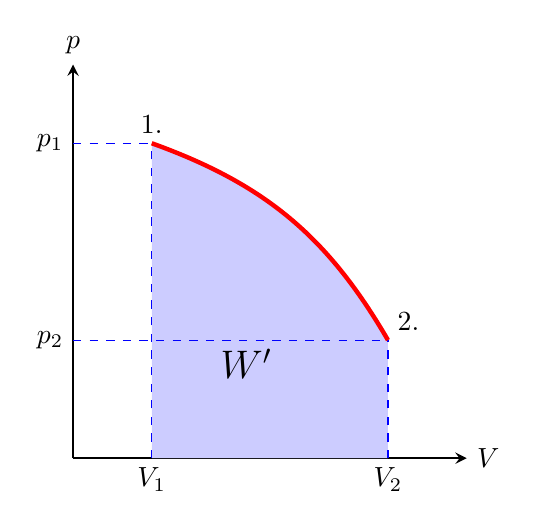
\begin{tikzpicture}[>=stealth]
    % Tengelyek
    \draw[->, thick] (0,0) -- (5,0) node[right] {$V$};
    \draw[->, thick] (0,0) -- (0,5) node[above] {$p$};

    % Pontok koordinátái
    \coordinate (1) at (1, 4);
    \coordinate (2) at (4, 1.5);

    % Világoskék kitöltés a görbe alatt (W')
    % A 'in' és 'out' szögek biztosítják, hogy a kitöltés széle ugyanaz a görbe legyen
    \fill[blue!20] (1,0) -- (1,4) to[bend left=20] (4,1.5) -- (4,0) -- cycle;
    \node at (2.2, 1.2) {\Large $W'$};

    % Szaggatott kék segédvonalak
    \draw[blue, dashed] (0,4) node[left, black] {$p_1$} -- (1);
    \draw[blue, dashed] (0,1.5) node[left, black] {$p_2$} -- (2);
    \draw[blue, dashed] (1,0) node[below, black] {$V_1$} -- (1);
    \draw[blue, dashed] (4,0) node[below, black] {$V_2$} -- (2);

    % Folyamat vonala (vastag vörös, enyhén görbe)
    \draw[red, ultra thick] (1) to[bend left=20] (2);

    % Pontok jelölése (1. és 2.)
    \node[above, black] at (1) {1.};
    \node[above right, black] at (2) {2.};

  \end{tikzpicture}
\end{center}
\end{column}
\end{columns}
  
\end{itemize}

\end{frame}

% ----------------------------------------------------------------------------------------------------------------------------------------

\begin{frame}%[fragile,squeeze,allowframebreaks]
\frametitle{Internal energy of ideal gas}

The internal energy of ideal gases (U) originates from

\begin{itemize}
\item Kinetic energy of particles ($E_{kinetic}$)
\item Potential energy of particles ($E_{potential}$)
\end{itemize}

Therefore,
$$U = E_{kinetic} + E_{potential}$$

Symbol: $U$

Unit: Joule (J)

\end{frame}

% ----------------------------------------------------------------------------------------------------------------------------------------

\begin{frame}[fragile,squeeze,allowframebreaks]
\frametitle{The first law of thermodynamics}

\begin{itemize}
\item \textbf{Conservation of energy}
\begin{itemize}
\item Macroscopic form:
$$ \Delta U = Q + W$$

%\item The change of internal energy ($\Delta U$) equals the heat (Q) transferred to the system plus the work (W) done on the system.

\item The energy of a thermodynamic system ($U$) is altered by the heat ($Q$) transferred to the system and the work ($W$) done on the system. In other words, the change in the system’s internal energy equals the sum of the heat transferred to the system and the work done on the system.
\item This stament expresses the law of conservation of energy in thermodynamics.
  
\smallskip

\item Microscopic form:
$$ dU = \delta Q + \delta W $$
\item $d$: the type of change (differential) is independent of the path (state function)
\item $\delta$: the type of change (differentials) depends on the path (path function)
\end{itemize}

\pagebreak
\item \textbf{Isochoric ($V = \text{const}$) process}
\begin{itemize}  
\item Volume does not change, hence
\vskip -20 pt
\begin{eqnarray*}
V &=& \text{const}\\
dV &=& 0 \\
\end{eqnarray*}
where $V$ is volume 
\item Therefore,
\vskip -20 pt
$$ dW = -p\, dV = 0,$$
where $W$ is work, $p$ is pressure.
\item The first law of thermodynamics in this case:
$$ dU = \delta Q + \delta W = \delta Q + 0 = \delta Q $$

\pagebreak
\item After integration:
$$dU=\delta Q \rightarrow U=Q $$

\item Internal energy:
\vskip -20 pt
\begin{eqnarray*}
U &=& c_V m T \\
\Delta U &=& c_{v} m \Delta T,
\end{eqnarray*}
\vskip -10 pt
where $m$ is mass, $\Delta T$ is temperature change, $c_{v}$ is specific heat coefficient at constant volume.
\end{itemize}

\pagebreak
\item \textbf{Isobaric  ($p = \text{const}$) process}
\begin{itemize}
\item Pressure ($p$) does not change
\vskip -15 pt
$$p = \text{const} $$
\vskip -20 pt
\item Elementary heat ($Q$, $\delta Q$):
\vskip -12 pt
$$ \delta Q = c_p m \Delta T \rightarrow Q = c_{p} m \Delta T,$$
\vskip -5 pt
where $m$ is mass, $\Delta T$ is temperature change, $c_{p}$ is specific heat coefficient at constant pressure.
\item The volume work (W) done on the gas by the surroundings:
  $$ W = -p\, dV, $$
where $p$ is pressure, $dV$ is volume change.
\end{itemize}

\pagebreak
\item \textbf{Definition (Enthalpy, H)}: Enthalpy is a state function, which is defined as the follows:
$$ H = U + pV,$$
where $U$ is energy, $p$ is pressure, $V$ is volume, furthermore $\left[H\right]=J$.
\begin{itemize}
\item From the first law of thermodynamics:
\vskip -20 pt
\begin{eqnarray*}
  dU &=& \delta Q + \delta W \\
  dU - \delta W &=& \delta Q \\
  dU - \left(p \cdot dV\right) &=& \delta Q
\end{eqnarray*}
\item We suppose that $p$=const, hence we can reorder for given heat the equation:
\vskip -20 pt
\begin{eqnarray*}
  dU + \left(p \cdot dV\right) &=& \delta Q \\
  d\left(U + pV\right) &=& \delta Q \\
  dH&=&\delta Q \text{\ \ differential form}
\end{eqnarray*}
\vskip -40 pt
\item Finally,
  $$dU=c_{p}\cdot m \cdot dT \rightarrow H=c_{p}\cdot m \cdot T.$$
\end{itemize}
\item Enthalpy is useful because, at constant pressure, the heat added to the system is exactly equal to the change in enthalpy. This is why it is used in chemistry and engineering to describe most reactions (those occurring in open vessels at atmospheric pressure).


\pagebreak
\item \textbf{Isothermal ($T=\text{conts}$) process}
\begin{itemize}
\item Temperature does not change
\vskip -15 pt
$$ T = \text{const} $$
\item Internal energy of ideal gas:
\vskip -15 pt
$$ dU = 0 \rightarrow \Delta U = 0$$
\item From the first law of thermodynamics:
\vskip -20 pt
\begin{eqnarray*}
dU &=& \delta Q + \delta W = 0 \\
\delta Q &=& -\delta W = p\cdot dV
\end{eqnarray*}
\item The volumetric work of the gas done by the surroundings on the gas:
\vskip -10 pt
$$W = -\frac{m}{M}RT \ln \left(\frac{V_{later}}{V_{earlier}}\right) = -\frac{m}{M}RT \ln \left(\frac{V_{2}}{V_{1}}\right)$$

\item Heat:
\vskip -22 pt
$$Q = -W = \frac{m}{M}RT \ln \left(\frac{V_{later}}{V_{earlier}}\right)= \frac{m}{M}RT \ln \left(\frac{V_{2}}{V_{1}}\right) $$

\end{itemize}

\pagebreak

\item \textbf{Definition (Adiabatic Process):} An adiabatic process is a thermodynamics process where there is no heat exchange between the gas and its surroundings ($Q=0$). 
\begin{itemize}
\item Internal energy of ideal gas: $dU=\delta Q +\delta W$, or $dU = 0 + \delta W = \delta W$.
\item For macroscopic quantities: 
$$\Delta U = W = c_V m \Delta T$$
\item \textbf{Definition (Specific heat ratio):} 
$$ \kappa = \frac{c_p}{c_V} = \frac{C_{p}}{C_{V}}$$

\pagebreak  
\item \textbf{Poisson formulas:} The equations below describe an \textbf{adiabatic process} for an ideal gas.
\begin{eqnarray*}
  p\cdot V^{\kappa}&=&\text{const}\\
  T\cdot V^{\kappa-1}&=&\text{const}\\
  T \cdot p^{\frac{1-\kappa}{\kappa}} &=& \text{const},
\end{eqnarray*}
where $p$ is pressure, $T$ is absolute temperature (K), $V$ is volume, and $\kappa$ (kappa) is heat capacity ratio ($c_p/c_v$).
\item Examples:
\begin{itemize}
\item \textbf{Adiabatic Compression:} If volume ($V$) decreases, the temperature ($T$) must increase (e.g., a bicycle pump getting warm).
\item \textbf{Adiabatic Expansion:} If volume ($V$) increases, the temperature ($T$) drops (e.g., the cooling effect of an aerosol spray).
\end{itemize}

\end{itemize}

\pagebreak
\item Curves of processes on the $p$-$V$ state diagram
\begin{center}
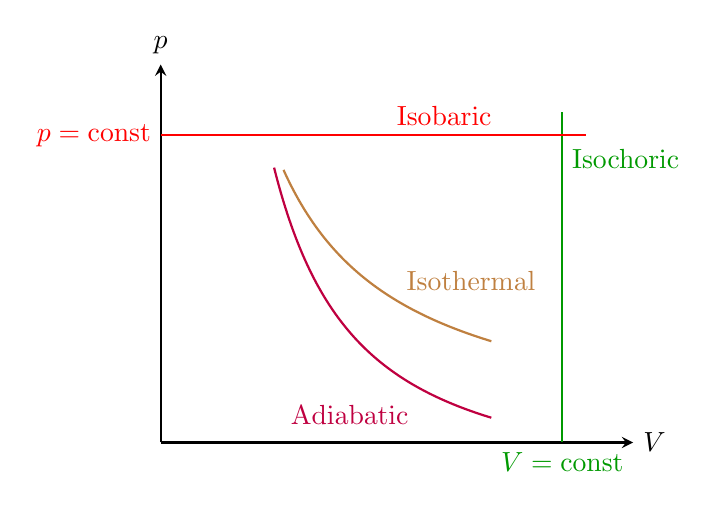
\begin{tikzpicture}[>=stealth, scale=1.2]
    % Tengelyek feketével, nyilakkal
    \draw[->, thick] (0,0) -- (5,0) node[right] {$V$};
    \draw[->, thick] (0,0) -- (0,4) node[above] {$p$};

    % Izochor (Zöld függőleges vonal)
    \draw[green!60!black, thick] (4.25, 0) -- (4.25, 3.5);
    \node[green!60!black, below] at (4.25, 0) {$V = \text{const}$};
    \node[green!60!black, right] at (4.25, 3) {Isochoric};

    % Izobár (Vörös vízszintes vonal)
    \draw[red, thick] (0, 3.25) -- (4.5, 3.25);
    \node[red, left] at (0, 3.25) {$p = \text{const}$};
    \node[red, above] at (3, 3.25) {Isobaric};

    % Metszéspont meghatározása a görbék indításához
    % (1.5, 2.5) a metszéspont
    
    % Izoterma (Barna görbe: p = k/V)
    % Úgy rajzoljuk, hogy átmenjen a metszésponton (1.5 * 2.5 = 3.75)
    \draw[brown, thick, domain=1.3:3.5, samples=100] plot (\x, {3.75/\x});
    \node[brown, above right] at (2.5, 1.5) {Isothermal};

    % Adiabata (Lila görbe: p = k/V^gamma)
    % Meredekebb, mint az izoterma. k = 2.5 * 1.5^1.4 ≈ 4.4
    \draw[purple, thick, domain=1.2:3.5, samples=100] plot (\x, {4.4/(\x^1.4)-0.5});
    \node[purple, below] at (2.0, 0.5) {Adiabatic};

\end{tikzpicture}
\end{center}

\end{itemize}

\end{frame}

% ----------------------------------------------------------------------------------------------------------------------------------------

\begin{frame}
%\frametitle{Minden jó, ha a vége jó}

\vfill
\begin{center}
\textbf{\huge The End}

\bigskip
Thank you for your attention!
\end{center}
\vfill
\textbf{Acknowledgements} Thank you for the course materials for Szilárd~ZSÓKA and Zoltán~VARGA.
\end{frame}

\end{document}
